%%%%%%%%%%%%%%%%%%%%%%%%%%%%%%%%%%%%%%%
% Ishan Tiwari - Resume
% 7/26/2016
%
% Reference:
% Debarghya Das (http://debarghyadas.com)

\documentclass[]{hieudo-build}

\usepackage[export]{adjustbox}
\begin{document}

%%%%%%%%%%%%%%%%%%%%%%%%%%%%%%%%%%%%%%
%
%     TITLE NAME
%
%%%%%%%%%%%%%%%%%%%%%%%%%%%%%%%%%%%%%%
%\begin{figure}
%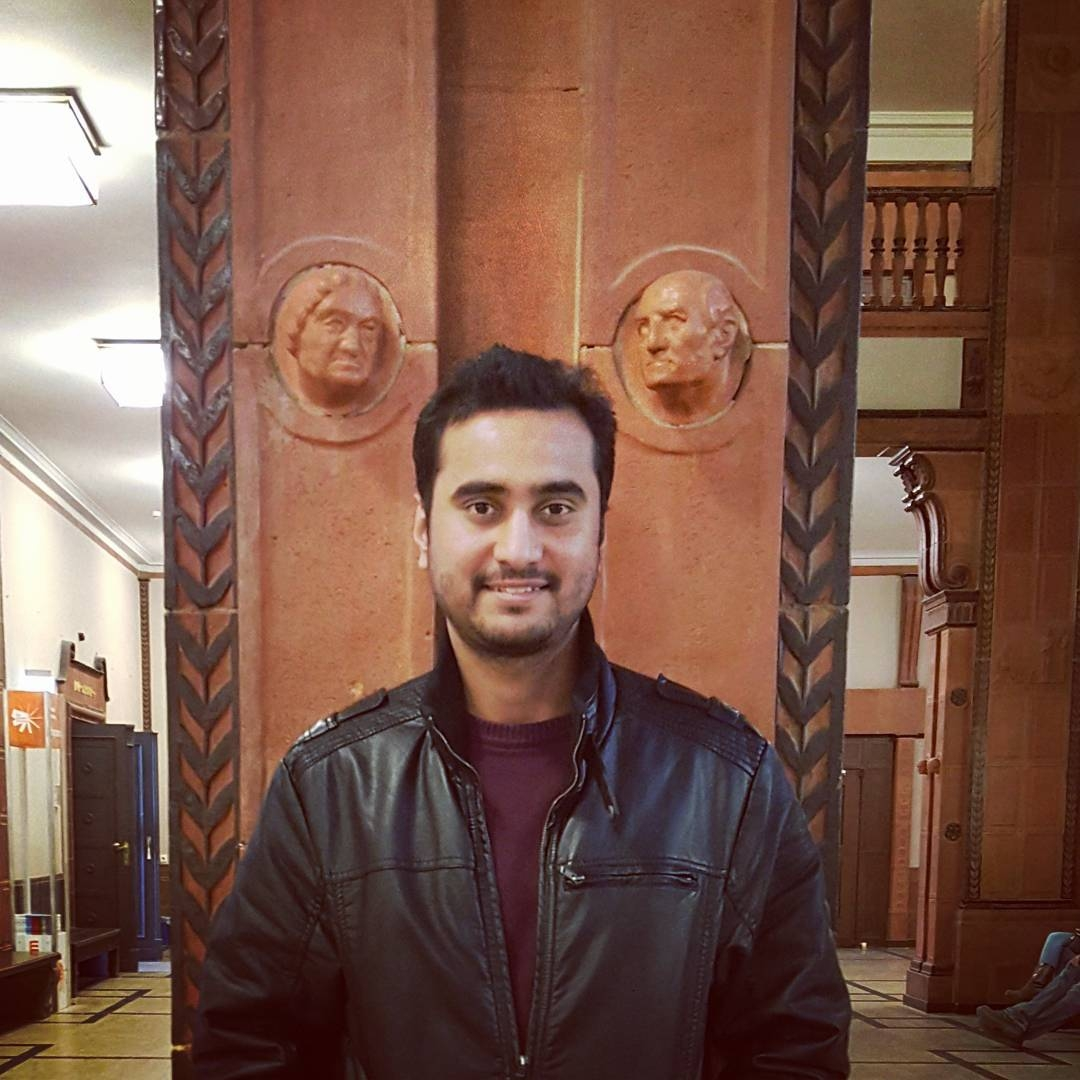
\includegraphics[width = .20\textwidth, left]{mypic}
%\end{figure}
\namesection{Ishan Tiwari}
{\urlstyle{same}
	\faEnvelope \href{mailto:ishan210788@gmail.com}{ ishan210788@gmail.com}\\
	\faGithub \href{https://github.com/ishantiw}{   github.com/ishantiw}\\
	\faLinkedinSquare \href{https://www.linkedin.com/in/ishantiwari}{ linkedin.com/in/ishantiwari}
}
    
%%%%%%%%%%%%%%%%%%%%%%%%%%%%%%%%%%%%%%
%
%     COLUMN ONE
%
%%%%%%%%%%%%%%%%%%%%%%%%%%%%%%%%%%%%%%
\begin{minipage}[t]{0.34\textwidth} 

%%%%%%%%%%%%%%%%%%%%%%%%%%%%%%%%%%%%%%
%     EDUCATION
%%%%%%%%%%%%%%%%%%%%%%%%%%%%%%%%%%%%%%
\section*{}
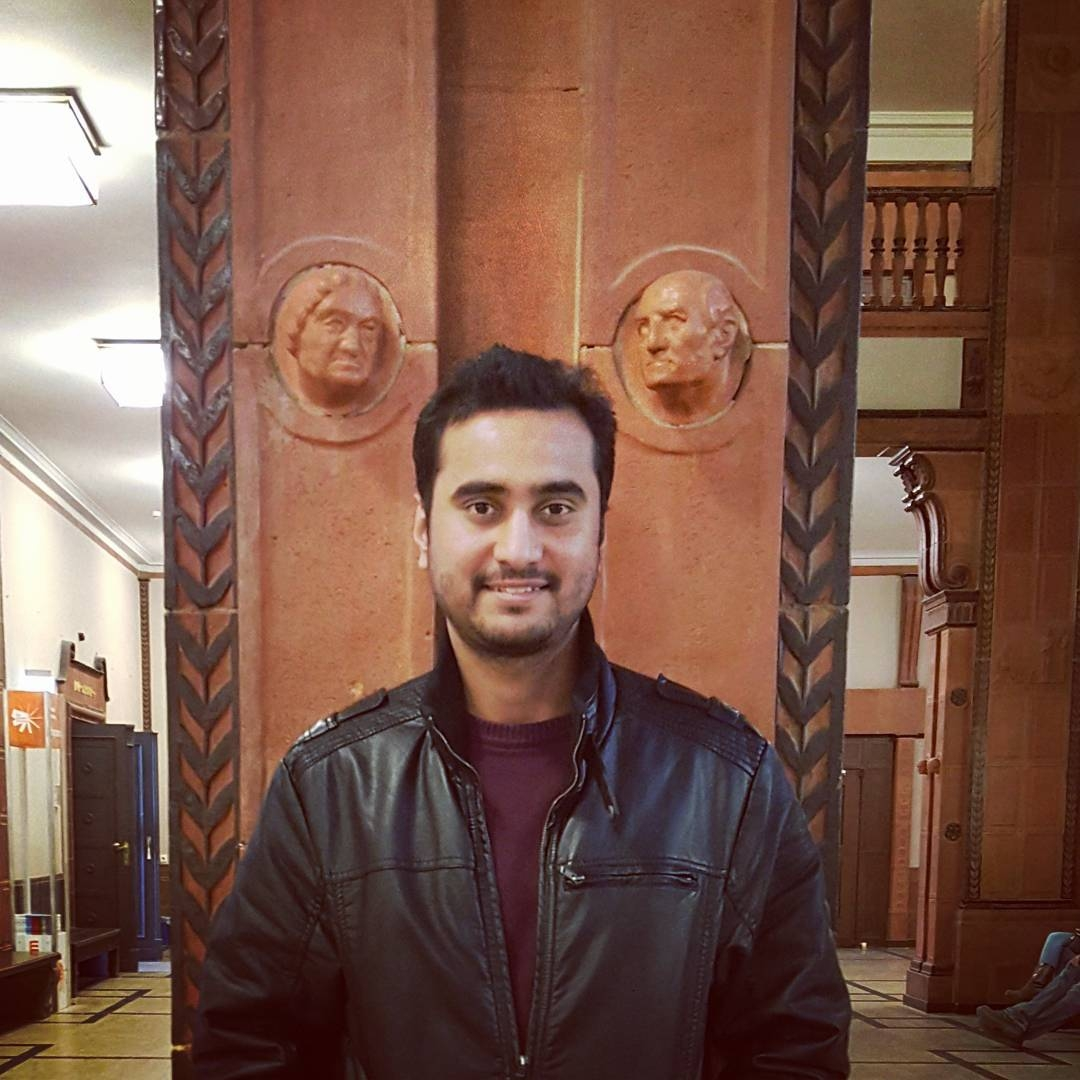
\includegraphics[width=0.75\textwidth]{mypic}
\linebreak
\_\_\_\_\faGithub \href{https://ishantiw.github.io}{ ishantiw.github.io}\_\_\_\_
\section{Education} 

\subsection{Technische Universität Berlin}
%\descript{Tandon School of Engineering}
Masters in Distributed Systems \\
and Services \\
Year 2015 - 2016 \\
Berlin, Germany \\
%Cum. GPA: 4.0\\
\sectionsep

\subsection{University College London}
Minor in Innovation and -\\ Entrepreneurship \\
June-July Year 2015\\
EIT Digital Masterschool, London \\
\sectionsep

\subsection{Université de Rennes 1}
Masters in Distributed Systems- \\
and Services, \\
Year 2014 - 2015, \\
Rennes, France \\
\sectionsep

\subsection{Uttaranchal Institute of Technology}
Bachelor of Technology - \\
in Computer Science\\
2007 - 2011 \\
Dehradun, India \\
\sectionsep

%%%%%%%%%%%%%%%%%%%%%%%%%%%%%%%%%%%%%%
%     SKILLS
%%%%%%%%%%%%%%%%%%%%%%%%%%%%%%%%%%%%%%
\section{Skills}
% \subsection{Programming}
\location{Core Languages Skills:}
JavaScript, Java, C\\ 

\location{Familiar with:}
C++, CUDA, Python(Django),\\
LaTeX, Hadoop

\location{Frameworks:}
NodeJS, MEANJS

\location{Databases:}
MongoDB, SQL, SQLlite, \\ Oracle Database \\

\location{Testing:}
Karma, JUnit, TDD, BDD

\location{Tools:}
Git, Docker,\\
Eclipse \& Apache Drill \\ 

% \sectionsep
% \subsection{Languages}
% \location{Native fluency:} English, Vietnamese\\
\sectionsep

% %%%%%%%%%%%%%%%%%%%%%%%%%%%%%%%%%%%%%%
% %     HACKATHONS
% %%%%%%%%%%%%%%%%%%%%%%%%%%%%%%%%%%%%%%
% \section{Hackathons}
% HackMIT \textbullet{} hackNY \\
% WearHacks NY \textbullet{} Hackademics VN \\
% \sectionsep


%%%%%%%%%%%%%%%%%%%%%%%%%%%%%%%%%%%%%%
%     COURSEWORK
%%%%%%%%%%%%%%%%%%%%%%%%%%%%%%%%%%%%%%

% \section{Coursework}
% Data Structure \\
% Algorithms \\
% Discrete Mathematics \\
% Artificial Intelligence \\
% Computer Architecture \\
% Computer Networking \\
% Data Analysis \\
% Object-Oriented Programming\\
% \sectionsep

%%%%%%%%%%%%%%%%%%%%%%%%%%%%%%%%%%%%%%
%     ADDITIONAL INFORMATION
%%%%%%%%%%%%%%%%%%%%%%%%%%%%%%%%%%%%%%
%\section{Activities}
%NYU Tandon Honors Program\\
%Tech@NYU - Freshman Circuit \\
%The Westminster News \\
%\sectionsep

% %%%%%%%%%%%%%%%%%%%%%%%%%%%%%%%%%%%%%%
% %     AWARDS
% %%%%%%%%%%%%%%%%%%%%%%%%%%%%%%%%%%%%%%

% \section{Awards} 
% Dean's List\\
% NYU PROMISE Scholarship\\
% Shelby C. Davis Scholarship\\
% President’s Circle Scholarship\\
% \sectionsep

\sectionsep
\DTMsetdatestyle{mylastupdate}
\DTMdisplaydate{\the\year}{\the\month}{\the\day}{-1}

%%%%%%%%%%%%%%%%%%%%%%%%%%%%%%%%%%%%%%
%
%     COLUMN TWO
%
%%%%%%%%%%%%%%%%%%%%%%%%%%%%%%%%%%%%%%
\end{minipage} 
\hfill
\begin{minipage}[t]{0.65\textwidth} 

%%%%%%%%%%%%%%%%%%%%%%%%%%%%%%%%%%%%%%
%     EXPERIENCE
%%%%%%%%%%%%%%%%%%%%%%%%%%%%%%%%%%%%%%
\section{Experience}

\workplace{Retail Media Group}{Apr 2017 – Present}\\
\position{Full Stack Developer}{Berlin, Germany}
\vspace{0.9em} % Hacky fix for awkward extra vertical space
\begin{tightemize}
\item Develop and maintenance of scalable micro service environments for big data. (Kubernetes Cluster, Nodejs, Mongodb, Redis)
\item Set up, gather and process raw data at scale (including writing scripts, web scraping, calling APIs, write SQL queries, etc.).
\item Process structured and unstructured data into a form suitable for analysis 
\item Working closely to our data science team
\item Implementing algorithms for data analysis
\end{tightemize}
\sectionsep

\workplace{T-Labs Deutsche Telekom}{Nov 2015 – Dec 2016}\\
\position{Student researcher}{Berlin, Germany}
\vspace{0.9em} % Hacky fix for awkward extra vertical space
\begin{tightemize}
\item Developing address book using NodeJS for \href{https://rethink-project.eu/}{reTHINK} for one of their use cases i.e., peer-to-peer social networking.
\item Integrating different components of reTHINK framework in order to make address book working and contributing to various repositories associated to these components. 
\item Research in P2P online social network including various attributes used for recommendations and testing them quantitatively.
\end{tightemize}
\sectionsep

\workplace{IGATE Global Solutions Limited (Capgemini)}{Jan 2012 – Apr 2014} \\
\position{Senior Software Engineer}{Mar 2013 – Apr 2014, Bangalore, India}
\position{Project - VARIABLE COMPENSATION PLAN (VCP)}{}
\position{Client - GE Healthcare}{}
% \vspace{\topsep} % Hacky fix for awkward extra vertical space
\begin{tightemize}
\item Development and testing various modules of VCP application using JSP, JavaScript \& Spring.
\item Created various documents related to client requirement, mappings and user training and writing procedures in Oracle for all the calculations related to Variable compensation.
\end{tightemize}
\sectionsep

\position{Software Engineer}{Jan 2012 – Feb 2013, Bangalore, India}
\position{Project - Emptoris Contract Management}{}
% \vspace{\topsep} % Hacky fix for awkward extra vertical space
\begin{tightemize}
\item Developing interview flows, contract, clause, users/user groups and approval rules and deployment of \href{https://www-01.ibm.com/software/info/emptoris/}{Emptoris Contract Management} for \href{www.gehealthcare.com/}{GE Healthcare} (Java, EJB and Web Logic).
\end{tightemize}
\sectionsep



% \runsubsection{The Westminster News} \\
% \descript{Co-Editors-in-Chief (2014) | Layout Editor (2012) }
% \location{Sep 2012 – May 2015 | Simsbury, CT}
% \begin{tightemize}
% \item Led 30+ staff at a 400-student boarding school to publish the monthly school newspaper.
% \item Consulted in layout design and technology application.
% \end{tightemize}
% \sectionsep

% \runsubsection{VietAbroader Organization} \\
% \descript{Program Assistant Manager | VAPedia Associate }
% \location{Mar 2013 – Mar 2014 | Ho Chi Minh City, Vietnam}
% \begin{tightemize}
% \item VietAbroader is a non-profit organization run by Vietnamese students abroad.
% \item Designed the high school content for the VAPedia website.
% \item Assisted in recruiting guest speakers and volunteers for VietAbroader Study-Abroad Conference 2013.
% \end{tightemize}
% \sectionsep

%%%%%%%%%%%%%%%%%%%%%%%%%%%%%%%%%%%%%%
%     PROJECTS
%%%%%%%%%%%%%%%%%%%%%%%%%%%%%%%%%%%%%%
\section{Projects}
\runsubsection{AIM1 project "NiteOut"}
\descript{}
\location{Technische Universität Berlin, Berlin 2016}
A web app to manage a group of events in an efficient way for a group of students in Berlin that takes real-world data of cinemas, transport, museums, etc from various data sources using MEAN STACK.

https://github.com/hielsnoppe/edu-aim1

\sectionsep

\runsubsection{Uncovering business opportunities from Yelp and OSM}
\descript{}
\location{Yelp Dataset Challenge 8th round}
Predicting success of a business at a location on a map.  Using location specific features, a heatmap is generated, which predicts the success of a location for a business type based on machine learning. We used Apache drill, NodeJS and LeafletJS.
\sectionsep 

\runsubsection{Google Transport API Parser}
\descript{}
\location{Technische Universität Berlin, Berlin 2015}
A module which parses the JSON data coming from Google transport API and provides various ways to display information (console, on map and object)

https://github.com/ishantiw/googleTransportAPIparser
\sectionsep



\end{minipage} 

\end{document}  
